%% Maurice Snoeren

%%
%% First part of the document
%%
\documentclass[9pt,a4paper]{report}
\usepackage[margin=1in]{geometry}
\usepackage[english]{babel}
\usepackage[utf8]{inputenc}
\usepackage{fancyhdr}
\usepackage{xcolor}
\usepackage{sectsty}
\usepackage{multirow}
\usepackage{amssymb}
\usepackage{xcolor}
\usepackage{array}
\usepackage{colortbl} % Required for coloring table cells
\usepackage[toc,page]{appendix}
\usepackage{seqsplit}% http://ctan.org/pkg/seqsplit

\usepackage{pdflscape} % Used for pdflatex change orientation
 
\usepackage[export]{adjustbox}
\usepackage{graphicx}
\usepackage{float} % used for H so that the figures stay inline of the text
\usepackage{longtable, array} % array for using m
\usepackage{enumitem} % Used for removing the margin top

\usepackage{pifont} % one block symbol

%% First use the Roman page numbering
%\pagenumbering{roman}

%% Change the fonts of the document to some sans serif type.
\renewcommand{\familydefault}{\sfdefault}

%% Define the Avans color of the headings
\definecolor{avansred}{RGB}{199,0,43}

%% Set the chapter numbering and toc depth level.
\setcounter{secnumdepth}{5} % seting level of numbering (default for "report" is 3). With ''-1'' you have non number also for chapters
%\setcounter{tocdepth}{2} % if you want all the levels in your table of contents

%% Change the title format
\usepackage{titlesec}

\titleformat{\chapter}[block]{\normalfont\huge\bfseries\color{avansred}}{\thechapter\enspace}{0.0em}{\huge}
\titlespacing{\chapter}{0.0em}{0.0em}{0.0em}

\titleformat{\section}[block]{\normalfont\bfseries\color{avansred}}{\thesection\enspace}{0.0em}{}
\titlespacing{\section}{0.0em}{1.0em}{0.0em}

\titleformat{\subsection}[block]{\normalfont\bfseries\color{avansred}}{\thesubsection\enspace}{0.0em}{}
\titlespacing{\subsection}{0.0em}{1.0em}{0.0em}

\titleformat{\subsubsection}[block]{\normalfont\bfseries\color{avansred}}{\thesubsubsection\enspace}{0.0em}{}
\titlespacing{\subsubsection}{0.0em}{1.0em}{0.0em}

\titleformat{\subsubsubsection}[block]{\normalfont\bfseries\color{avansred}}{\thesubsubsubsection\enspace}{0.0em}{}
\titlespacing{\subsubsubsection}{0.0em}{1.0em}{0.0em}

%% Change the title of the Table of contents
\addto\captionsenglish{% Replace "english" with the language you use
  \renewcommand{\contentsname}%
    {Table of contents}%
}

%% Change the header and footer according to the Avans template
\pagestyle{fancy}
\fancyhf{}
\lhead{
\includegraphics[width=1.00\textwidth,height=10.0mm]{images/avans-bar.png}
\includegraphics[width=40.0mm,right]{images/avans-logo.png}}
\lfoot{\footnotesize{Avans Hogeschool - \ReportTitle - \CourseCode - www.avans.nl}}
\rfoot{\footnotesize{Page \thepage}}
\renewcommand{\headrulewidth}{0pt}
\renewcommand{\footrulewidth}{1pt}

\fancypagestyle{plain} { %The chapter and table of contents reset to the plain style, therefore redefined it.
 \pagestyle{fancy}
}

\usepackage[absolute]{textpos}
\usepackage{booktabs}
\fancypagestyle{lscape} { %
 \fancyhf{} % clear all header and footer fields
 \fancyfoot[L] {
 \begin{textblock}{1}(19.75,3.5){\rotatebox{90}{\footnotesize{Page \thepage}}}\end{textblock} % this positions the page number
 \begin{textblock}{24.5}(19.60,3.5){\rotatebox{90}{\rule{\textwidth}{1.0pt}}}\end{textblock} % this positions the page number
 \begin{textblock}{24.5}(19.75,16.5){\rotatebox{90}{\footnotesize{Avans Hogeschool - \ReportTitle - \CourseCode - www.avans.nl}}}\end{textblock}
 \begin{textblock}{20}(1.0,7.9){\rotatebox{90}{
\includegraphics[width=1.00\textwidth,height=10.0mm]{images/avans-bar.png}}}\end{textblock}}

 \setlength{\TPHorizModule}{1cm}
 \setlength{\TPVertModule}{1cm}
 \renewcommand{\headrulewidth}{0.0pt}
 \renewcommand{\footrulewidth}{0.0pt}
}

\fancypagestyle{nofoot} { % Define a new page style for the first and last page without a footer and with a different header
 \fancyhf{} % Clear all header and footer fields 
\lhead{
 
\includegraphics[width=1.00\textwidth,height=10.0mm]{images/avans-bar.png}
 
\includegraphics[width=40.0mm,right]{images/avans-logo.png}
}
 \renewcommand{\headrulewidth}{0pt}
 \renewcommand{\footrulewidth}{0pt}
}

% No indent please!
\setlength\parindent{0pt}



% Use to mark your document as draft!
%\usepackage{draftwatermark}
%\SetWatermarkText{DRAFT}
%\SetWatermarkScale{8}

%----------------------------------------------------------------------------------------
%	CUSTOM COMMANDS
%----------------------------------------------------------------------------------------

\newcommand{\DateofIssue}[1]{\renewcommand{\DateofIssue}{#1}}
\newcommand{\ReportNumber}[1]{\renewcommand{\ReportNumber}{#1}}
\newcommand{\Revision}[1]{\renewcommand{\Revision}{#1}}

\newcommand{\DepartmentName}[1]{\renewcommand{\DepartmentName}{#1}}
\newcommand{\ReportTitle}[1]{\renewcommand{\ReportTitle}{#1}}
\newcommand{\CourseCode}[1]{\renewcommand{\CourseCode}{#1}}
\newcommand{\AuthorName}[1]{\renewcommand{\AuthorName}{#1}}
\newcommand{\AuthorEmail}[1]{\renewcommand{\AuthorEmail}{#1}}
\newcommand{\Version}[1]{\renewcommand{\Version}{#1}}

%----------------------------------------------------------------------------------------
%	REPORT META-INFORMATION
%----------------------------------------------------------------------------------------

\DepartmentName{Academie voor Engineering \& ICT}
\AuthorName{Automatisch gegenereerd}
\AuthorEmail{mac.snoeren@avans.nl}
\DateofIssue{2018-11-14}
\Version{1.0}
\Revision{0}



%----------------------------------------------------------------------------------------
%	END OF REPORT META-INFORMATION
%----------------------------------------------------------------------------------------


\CourseCode{TMTI-OGP2}
\ReportTitle{Tentamen resultaten OGP2}

\begin{document}

%%----------------------------------------------------------------------------------------
%	COVER PAGE
%----------------------------------------------------------------------------------------

\begin{titlepage}
  \centering
  
\includegraphics[width=1.00\textwidth,height=10.0mm]{images/avans-bar.png}
  
\includegraphics[width=40.0mm,right]{images/avans-logo.png}

  \vfill

  \begin{flushleft}{\fontsize{13pt}{19.5pt}\selectfont\MakeUppercase{\textbf{\DepartmentName}}}\end{flushleft} 
  \begin{flushleft}{\fontsize{28pt}{42pt}\selectfont\color{avansred}\textbf{\ReportTitle}}\end{flushleft}
  \begin{flushleft}{\fontsize{14pt}{21pt}\selectfont\textbf{\CourseCode}}\end{flushleft}

  \vfill

  \begin{flushleft}{\textbf{Author(s):} \AuthorName}\\[4pt]\end{flushleft}
  \begin{flushleft}{\textbf{Date:} \DateofIssue}\end{flushleft}
  \begin{flushleft}{\textbf{Versie:} \Version}\\[4pt]\end{flushleft}

  \vfill

  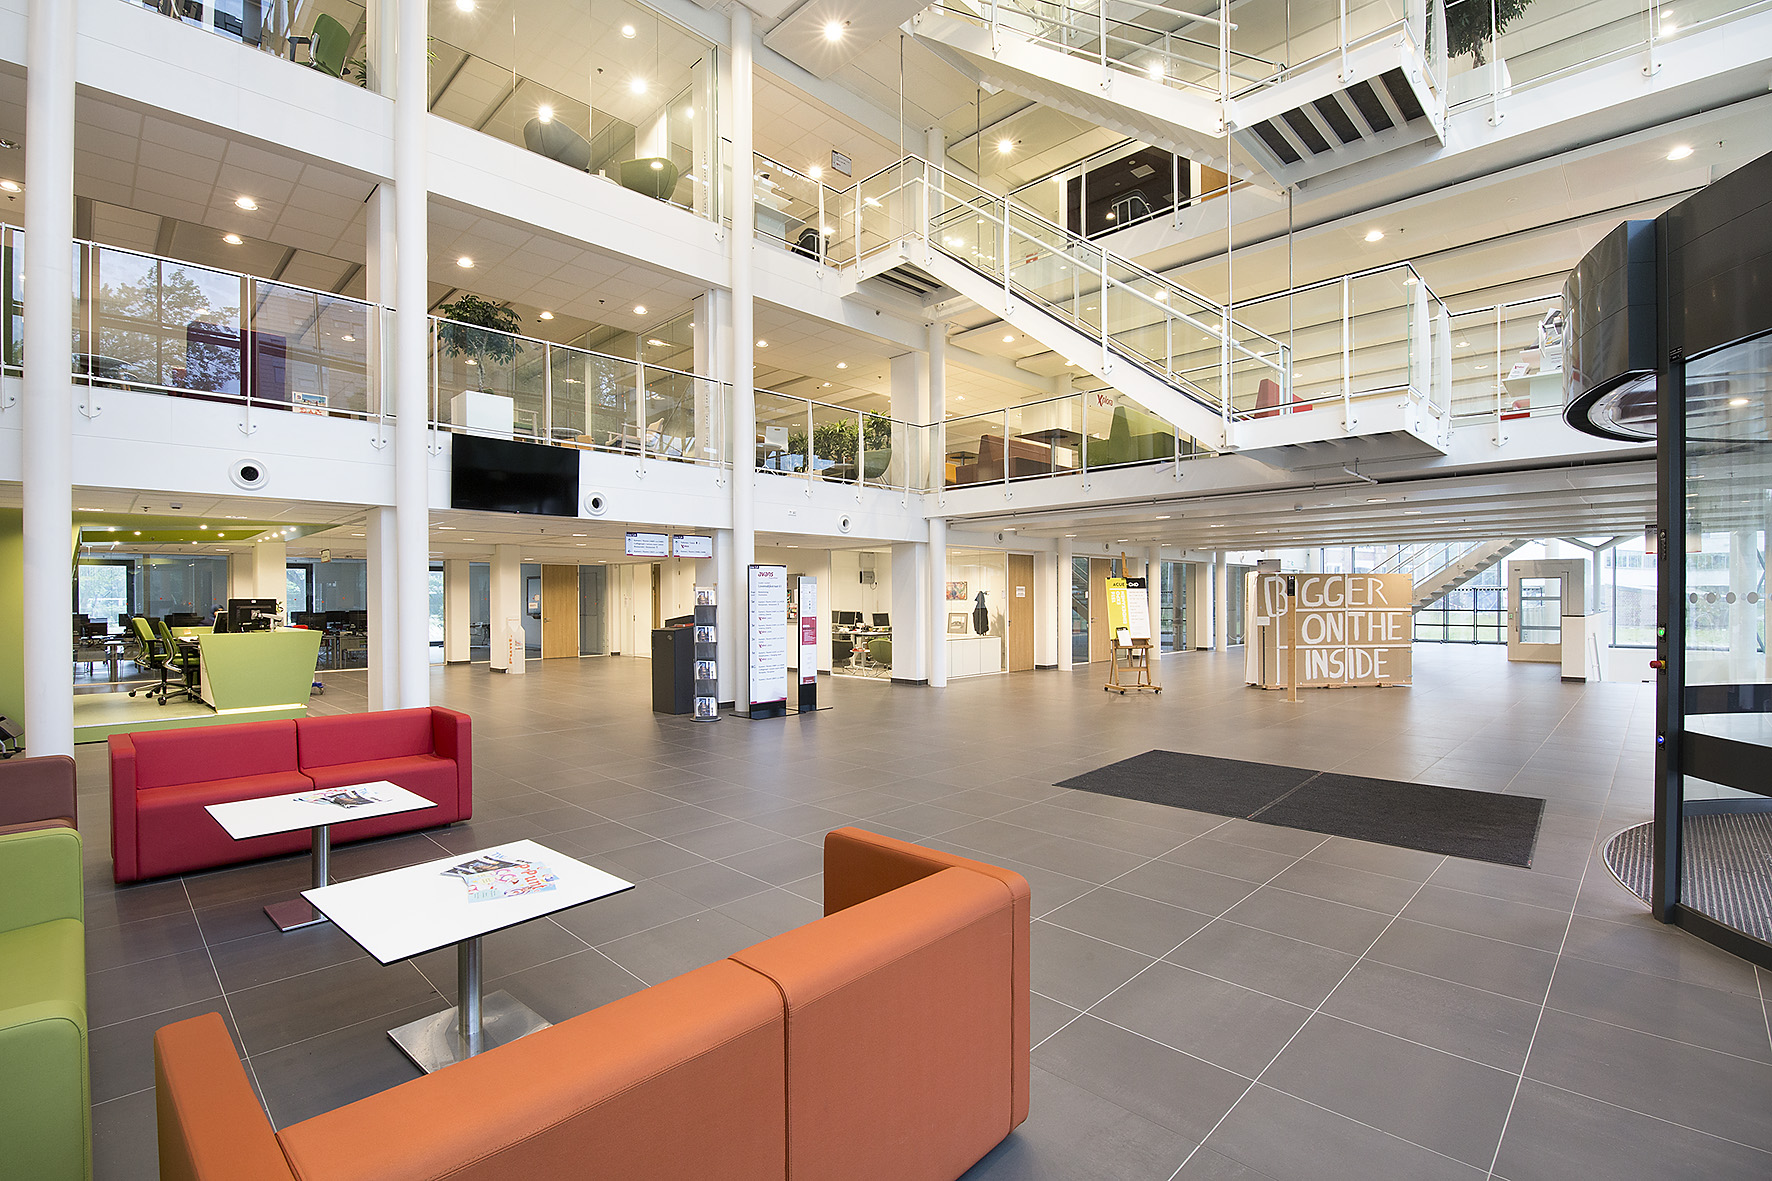
\includegraphics[width=1.00\textwidth]{images/avans-foto.jpg}

\end{titlepage}

%----------------------------------------------------------------------------------------
%	END COVER PAGE
%----------------------------------------------------------------------------------------


%$%----------------------------------------------------------------------------------------
%	TITLE PAGE
%----------------------------------------------------------------------------------------

\vspace*{0.5cm}

\begin{table}[h]
\begin{tabular}{@{}lp{5cm}l@{}}
Course & : \ReportTitle & Avans Hogeschool\\
Code & : \CourseCode & \DepartmentName\\
Docent(en) & : \AuthorName & 4800 RA Breda \\
Email & : \AuthorEmail & Postbus 90.116\\
Datum & : \DateofIssue & \\
Versie & : \Version & \\
\end{tabular}
\end{table}

\vspace{0.5cm}

\rule{\textwidth}{0.4pt}

\begin{table}[h]
\fontsize{7pt}{8.5pt}\selectfont
\begin{tabular}{@{}p{0.3\linewidth}@{}p{0.05\linewidth}@{}p{0.3\linewidth}@{}p{0.05\linewidth}@{}p{0.3\linewidth}@{}}
\normalsize{Geschreven door:} && \normalsize{Nagekeken door:} && \normalsize{Goedgekeurd door:}\\[50pt]
%\includegraphics[width=0.3\textwidth]{images/robin.png} \hrule && \includegraphics[width=0.3\textwidth]{images/maurice.png} \hrule && \hrule \\[-0pt] 
 \hrule && \hrule && \hrule \\[-0pt] 
{Maurice Snoeren} && {Diederich Kroeske} && {Jessica van der Heijden}\\[10pt]
{Docent} && {Docent} && {Team Opleiding Co\"ordinator}\\[10pt]
\end{tabular}
\end{table}

\vfill

\rule{\textwidth}{0.4pt}
{\fontsize{8pt}{10.5pt}\selectfont Copyright \copyright  Avans Hogeschool 2018. All rights reserved. Unless otherwise
agreed in writing.

\vspace{0pt}

\rule{\textwidth}{0.4pt}

\begin{table}[!h]
\fontsize{7pt}{8.5pt}\selectfont
\begin{tabular}{p{0.14\linewidth}p{0.14\linewidth}p{0.14\linewidth}p{0.14\linewidth}p{0.14\linewidth}p{0.14\linewidth}@{}}
\rowcolor{avansred} Versie & Datum & Aanpassingen & Gemaakt & Nagekeken & Goedgekeurd\\
%1 & 2017-11-28 & First issue
\end{tabular}
\end{table}

\vfill

{\fontsize{8pt}{10.5pt}\selectfont Avans Hogeschool}

\fontsize{10}{14}\selectfont

%----------------------------------------------------------------------------------------
%	END TITLE PAGE
%----------------------------------------------------------------------------------------


%\chapter*{Executive summary}

<< Please put here your executive summary >>


\pagestyle{fancy}

\setcounter{tocdepth}{0}
%$\tableofcontents
 
%\chapter{Introduction}
\pagenumbering{arabic}

< Introduction comes here...>

\chapter{Student: @Model.student.name}
\begin{longtable}[h]{|p{.25\textwidth}|p{.25\textwidth}|p{.25\textwidth}|p{.25\textwidth}|}
\hline
Studentnummer: @Model.student.number & Naam: @Model.student.name & Nagekeken door: @Model.ManualCorrector & Cijfer: @Model.Grade (@Model.TotalPoints punten) \\
\hline
\end{longtable}


@if(Model.mc.Count > 0) {
@:\section{Theorie multiple choice (@Model.mcTotalPoints punten)}
@:\begin{longtable}[h]{|l|@foreach(var q in Model.mc) {<text>l|</text>}}
@:\hline
@:Vraag @foreach(var q in Model.mc) {<text> & @q.question</text>} \\
@:\hline
@:Jouw antwoord @foreach(var q in Model.mc) {<text> & @q.answer</text>} \\
@:\hline
@:Correcte antwoord @foreach(var q in Model.mc) {<text> & @q.correctanswer</text>} \\
@:\hline
@:Punten @foreach(var q in Model.mc) {<text> & @q.score</text>} \\
@:\hline
@:\end{longtable}
}



\section{Theorie open vragen (5 punten)}
\begin{longtable}[h]{|l|l|p{.55\textwidth}|}
\hline
Vraag & Punten & Uitleg \\
\hline
@foreach(var q in Model.open)
{
@:@q.question & @q.score & @q.reason \\
@:\hline
}
\end{longtable}





\section{Praktijk (100 punten)}
\begin{longtable}[h]{|l|l|l|>{\raggedright\arraybackslash}p{.25\textwidth}|>{\raggedright\arraybackslash}p{.55\textwidth}|}
\hline
Vraag & Test & Corr. & Uitleg & Test foutmelding \\
\hline
@foreach(var q in Model.questions)
{
@:@q.question & @q.testScore & @q.manualScore & @q.manualReason & @q.testErrors \\
@:\hline
}

\end{longtable}


%\input{chapters/conclusions.tex}

%\input{chapters/glossary.tex}

%\begin{appendices}

%\input{chapters/appendix-a.tex}

%\input{chapters/appendix-b.tex}


%\end{appendices}

%%
%% Last part of the document
%%
%$
%----------------------------------------------------------------------------------------
%	DISCLAIMER
%----------------------------------------------------------------------------------------

\newpage

\thispagestyle{nofoot}

~\vfill




\textcolor{avansred}{\textbf{\fontsize{13pt}{19.5pt}\selectfont Organisatie Avans Hogeschool}}

Avans Hogeschool is in 2004 ontstaan door een fusie tussen Hogeschool Brabant en Hogeschool Brabant en 's-Hertogenbosch. Deze kennisinstituten werkten toen al nauw samen onder \'{e}\'{e}n Collega van Bestuur.

\

\textcolor{avansred}{\textbf{\fontsize{13pt}{19.5pt}\selectfont Academies}}

De opleidingen zijn verdeeld over 21 academies. Inclusief de Juridische Hogeschool Avans-Fontys. Wij hebben academies in de interessegebieden Economie en Bedrijf, Techniek, Gedrag en Maatschappij, Gezondheid, Exact en Informatica, Kunst en Cultuur, Recht en Bestuur, Onderwijs en Opvoeding, Aarde en milieu en Taal en Communicatie.

\

\textcolor{avansred}{\textbf{\fontsize{13pt}{19.5pt}\selectfont Onderzoek}}

Avans heeft 6 expertisecentra en ruim 25 lectoraten voor onderzoek. Groepen onderzoekers die praktijkgericht onderzoek doen.

\

\textcolor{avansred}{\textbf{\fontsize{13pt}{19.5pt}\selectfont Disclaimer}}

Aan dit rapport, waaronder ook de eventuele bijlagen worden bedoeld, kunnen geen rechten worden ontleend. Het is niet toegestaan om dit repport, geheel of gedeeltelijk, zonder toestemming te gebruiken of te verspreiden. Avans Hogeschool sluit elke aansprakelijkheid uit wanneer informatie in dit rapport niet correct, onvolledig of niet tijdig overkomt.

\

\



\end{document}
